\documentclass{homework}

\usepackage{subfig}
\usepackage{multicol}
\usepackage{float}
\usepackage{bookmark}
\usepackage{hyperref}
\usepackage{xcolor}
\usepackage{listings}
\lstset{literate=
	{á}{{\'a}}1 {é}{{\'e}}1 {í}{{\'i}}1 {ó}{{\'o}}1 {ú}{{\'u}}1
	{Á}{{\'A}}1 {É}{{\'E}}1 {Í}{{\'I}}1 {Ó}{{\'O}}1 {Ú}{{\'U}}1
	{à}{{\`a}}1 {è}{{\`e}}1 {ì}{{\`i}}1 {ò}{{\`o}}1 {ù}{{\`u}}1
	{À}{{\`A}}1 {È}{{\'E}}1 {Ì}{{\`I}}1 {Ò}{{\`O}}1 {Ù}{{\`U}}1
	{ä}{{\"a}}1 {ë}{{\"e}}1 {ï}{{\"i}}1 {ö}{{\"o}}1 {ü}{{\"u}}1
	{Ä}{{\"A}}1 {Ë}{{\"E}}1 {Ï}{{\"I}}1 {Ö}{{\"O}}1 {Ü}{{\"U}}1
	{â}{{\^a}}1 {ê}{{\^e}}1 {î}{{\^i}}1 {ô}{{\^o}}1 {û}{{\^u}}1
	{Â}{{\^A}}1 {Ê}{{\^E}}1 {Î}{{\^I}}1 {Ô}{{\^O}}1 {Û}{{\^U}}1
	{ã}{{\~a}}1 {ẽ}{{\~e}}1 {ĩ}{{\~i}}1 {õ}{{\~o}}1 {ũ}{{\~u}}1
	{Ã}{{\~A}}1 {Ẽ}{{\~E}}1 {Ĩ}{{\~I}}1 {Õ}{{\~O}}1 {Ũ}{{\~U}}1
	{œ}{{\oe}}1 {Œ}{{\OE}}1 {æ}{{\ae}}1 {Æ}{{\AE}}1 {ß}{{\ss}}1
	{ű}{{\H{u}}}1 {Ű}{{\H{U}}}1 {ő}{{\H{o}}}1 {Ő}{{\H{O}}}1
	{ç}{{\c c}}1 {Ç}{{\c C}}1 {ø}{{\o}}1 {å}{{\r a}}1 {Å}{{\r A}}1
	{€}{{\euro}}1 {£}{{\pounds}}1 {«}{{\guillemotleft}}1
	{»}{{\guillemotright}}1 {ñ}{{\~n}}1 {Ñ}{{\~N}}1 {¿}{{?`}}1 {¡}{{!`}}1 
}

\definecolor{codegreen}{rgb}{0,0.6,0}
\definecolor{codegray}{rgb}{0.5,0.5,0.5}
\definecolor{codepurple}{rgb}{0.58,0,0.82}
\definecolor{backcolour}{rgb}{0.95,0.95,0.95}

\lstdefinestyle{mystyle}{
	backgroundcolor=\color{backcolour},   
	commentstyle=\color{codegreen},
	keywordstyle=\color{blue},
	numberstyle=\tiny\color{codegray},
	stringstyle=\color{codepurple},
	basicstyle=\ttfamily\footnotesize,
	breakatwhitespace=false,         
	breaklines=true,                 
	captionpos=b,                    
	keepspaces=true,                 
	numbers=left,                    
	numbersep=5pt,                  
	showspaces=false,                
	showstringspaces=false,
	showtabs=false,                  
	tabsize=2,
	xleftmargin=.25in
}

\lstset{style=mystyle}

\title{Práctica 1: Análisis de Eficiencia de Algoritmos}
\author{Shao Jie Hu Chen \\ Mario Megías Mateo \\ Jesús Samuel García Carballo}
\renewcommand{\course}{Algorítmica}
\date{1 de abril de 2022}

\begin{document}
	\maketitle

    \newpage

    \begin{abstract}
		Esto es una prueba
	\end{abstract}
	
    \newpage

	\tableofcontents
	\newpage
	\setcounter{page}{1}
	
	\section{Introducción}

    En esta primera práctica de la asignatura Algorítmica vamos a realizar un análisis teórico y empírico de
    diversos algoritmos vistos en la asignatura. En particular, dicho análisis se hará de los siguientes:

    \begin{itemize}
        \item \textbf{Algoritmos de ordenación:} Inserción, selección, quicksort y mergesort. 
        \item \textbf{Algoritmo de análisis de caminos mínimos sobre grafos:} Algoritmo de Floyd.
        \item \textbf{Hanoi.} Resolución del juego de las torres de Hanoi. 
    \end{itemize}

    \subsection{Estructura de la memoria}
    
	Esta memoria presenta la estructura típica de un trabajo académico. En primer lugar, presentamos
    brevemente el contexto en el que nos manejamos en esta práctica. Posteriormente, analizaremos teóricamente
    cada uno de los algoritmos propuestos para, seguidamente, comprobar mediante un 
    análisis empírico las soluciones obtenidas. Asimismo, se ha realizado un análisis híbrido contrastando
    los resultados teóricos con los experimentales. Este análisis se ha realizado para cada algoritmo, 
    extrayéndose información relevante asociada a ellas. 
    
    Además, para cada uno de los algoritmos considerados, se ha
    elaborado conjuntamente entre los miembros del grupo tablas asociadas a cada una de ellas, que se
    irán presentando a lo largo de esta memoria. Finalmente, se escribirán unas
    líneas asociadas a las conclusiones obtenidas tras el desarrollo de esta práctica, así como los resultados
    más relevantes obtenidos. 

    \subsection{Objetivos} 

    Entre los objetivos que vamos a realizar asociadas a esta práctica, caben destacar los siguientes: 

    \begin{itemize}
        \item \textbf{Estudio teórico, empírico e híbrido} y \textbf{comparación} de los algoritmos de ordenación más empleados, verificando los resultados teóricos.
        \item \textbf{Estudio teórico, empírico e híbrido} de algoritmos de alta complejidad, poniendo especial énfasis en su \textbf{viabilidad} en diferentes equipos. 
        \item Estudio del \textbf{aumento de eficiencia} de un mismo algoritmo para diferentes \textbf{tipos de optimización} del compilador. 
        \item Determinación del algoritmo \textbf{más adecuado} para cada situación en función del estado de los datos.
    \end{itemize}

    \subsection{Equipo empleado}

    Para el desarrollo de esta práctica, se han empleado diferentes equipos, cuyas respectivas especificaciones técnicas se 
    especifican a continuación:
    
    \begin{itemize}
        \item \textbf{ASUS} 
        \begin{itemize}
            \item \textbf{Modelo}: ZenBook 15 UX534F
            \item \textbf{Procesador}: Intel(R) Core(TM) i7-10510U CPU @ 1.80GHz5
            \item \textbf{Memoria Ram}: 16 GB DDR4 @ 2.133 MHz.
            \item \textbf{Sistema Operativo} Ubuntu 20.04.2 LTS
        \end{itemize}
        
        \item \textbf{LENOVO}
        \begin{itemize}
            \item \textbf{Modelo}: YOGA 530-14IKB
            \item \textbf{Procesador}: Intel(R) Core(TM) i5-8250U CPU @ 1.60GHz
            \item \textbf{Memoria RAM:} 8 GB DDR4
            \item \textbf{Sistema Operativo}: Ubuntu 20.04.4 LTS
        \end{itemize}
        
        \item \textbf{HP}
        \begin{itemize}
            \item \textbf{Modelo}: HP Pavilion Gaming Laptop 15-dk0xxx
            \item \textbf{Procesador}: Intel(R) Core(TM) i7-9750H CPU @ 2.60GHz
            \item \textbf{Memoria RAM:} 32 GB DDR4
            \item \textbf{Sistema Operativo}: Ubuntu 20.04.4 LTS
        \end{itemize}
    \end{itemize}
    
    Debido a las limitaciones técnicas de estos equipos, para el cálculo de la eficiencia empírica se ha 
    optado por medir tiempos de ejecución en tiempos y \textbf{tamaños razonables} para obtener datos relevantes
    para el comportamiento tanto a pequeñas escalas como a nivel asintótico de ellas. 

    \section{Eficiencia teórica}

    Para el análisis de los siguientes algoritmos se ha empleado la notación $O(.)$. 

    \subsection{Algoritmo de inserción}

    El código de este algoritmo lo podemos encontrar a continuación.

    \lstinputlisting[language=C++, firstline=66, lastline=79, caption=Implementación en C++ del algoritmo de inserción.]{../src/insercion.cpp}
    
    El análisis de eficiencia se ha de hacer sobre el número de elementos del vector $n$. 

    Para el análisis asintótico, calculamos el número de operaciones elementales asociadas al código. 
    Las tres primeras líneas tienen complejidad $O(1)$. Para el ciclo for, démonos cuenta de que itera sobre el número de
    componentes del vector. Por su parte, dentro del for existe un while que realiza un conjunto de operaciones de orden
    $O(1)$ tantas veces como se indica en el iterador. Por tanto, llamando $T(n)$ al números de operaciones asociadas
    al algoritmo, tenemos que:

    \begin{equation*}
        T(n) = \sum_{i=0}^{n-1} \sum_{j=0}^{i-1} k = \sum_{i=0}^{n-1} ki = k \frac{n(n-1)}{2} 
    \end{equation*}

    Por tanto, deducimos que $T(n) \in O(n^2)$. 

    \subsection{Algoritmo de selección}

    \lstinputlisting[language=C++, firstline=66, lastline=82, caption=Implementación en C++ del algoritmo de selección.]{../src/seleccion.cpp}    

    La estructura principal del código anterior consta de dos bucles for anidados. Las primeras sentencias de declaración antes del inicio del primer 
    bucle for no repercuten en el análisis. Procedamos a analizar la estructura repetitiva: el primer for recorre el vector desde su inicio hasta
    la penúltima componente del mismo incluída. El segundo for comienza en la posición dada por el índice del primero hasta la última componente del vector incluída.
    Dentro del bucle interno tenemos una operación elemental correspondiente a la comparación realizada en el if, que es $O(1)$. Dentro del bucle externo excluyendo 
    el código del bucle interno nos encontramos con dos sentencias de asignación que no se tendrán en cuenta para el análisis. De igual modo, fuera del bucle externo
    al final del código nos encontramos con otras sentencias de asignación que también serán despreciadas. También tendremos en cuenta las operaciones elementales
    aritméticos correspondientes a la gestión de los bucles, que son $O(1)$. En conclusion, acotando las expresiones $O(1)$ por k tenemos que: 

    \begin{equation*}
        \begin{split}
            T(n) = \sum_{i=0}^{n-2} \sum_{j=i}^{n-1} k = \sum_{i=0}^{n-2} k(n-1-i+1) = \sum_{i=0}^{n-2} k(n-i) = kn \sum_{i=0}^{n-2} 1  - k \sum_{i=0}^{n-2} i \\
            = kn(n-2+1) - k \frac{(n-2)(n-1)}{2} = kn^2 + kn - \frac{kn^2 - 3kn + 2k}{2}
        \end{split}
    \end{equation*}
    
    Deducimos, por tanto, que $T(n) \in O(n^2)$. 
    
    \subsection{Algoritmo HeapSort}
    
    \lstinputlisting[language=C++, firstline=59, lastline=71, caption=Implementación en C++ del algoritmo heapsort.]{../src/heapsort.cpp} 

    El heapsort es un algoritmo de ordenación por montículos que consta de dos bucles for independientes, que llaman a una función llamada reajustar.
    En la primera línea de código podemos encontrar una declaración de variable cuya eficiencia es $O(1)$ y luego los dos ciclos mencionados, que interan 
    sobre el número de elementos del vector que denotaremos por $n$, luego realizaremos la eficiencia en torno a este dato. Ambos ciclos son independientes, 
    así que vamos a analizar cada uno por separado y aplicando la regla del máximo nos quedaremos con el mayor.
    
    La función reajustar trata de imitar el uso de un árbol APO mediante vectores y recorrerlo insertando elementos, luego como en un árbol APO la inserción se 
    realiza con eficiencia $O(log_2(n))$. Así que respecto a ambos ciclos tenemos lo siguiente:
    
    \begin{itemize}
        \item \textbf{Primer ciclo}
        \begin{equation*}
            T(n) = \sum_{i=0}^{n/2 + 1} log_2(k) = ((n/2 +1)*(n/2 + 2))/2 * log_2(k) \in O(n*log(n))
        \end{equation*} 

        \item \textbf{Segundo ciclo}
        \begin{equation*}
            T(n) = \sum_{i=1}^{n-1} log_2(k) = (((n-1)*n)/2) * log_2(n). \in O(n*log(n))
        \end{equation*}
        
    \end{itemize}

    \subsection{Algoritmo QuickSort}
    
    \lstinputlisting[language=C++, firstline=141, lastline=184, caption=Implementación en C++ del algoritmo QuickSort.]{../src/quicksort.cpp} 

    En este apartado, consideramos $n$ como el número de componentes del vector. 

    El código del algoritmo comienza en la función quicksort\_lims en la línea 6. Tomaremos inicial 
    como ñaa posición de comienzo del vector ($inicial = 0$), y final como el siguiente al último elemento, 
    que coincide con el número de componentes del vector ($final = n$).
    Tenemos una estructura condicional que determina el comportamiento del algoritmo según si el tamaño del vector 
    supera o no un cierto umbral, por lo que el tiempo de ejecución será una función definida a trozos. Si es menor 
    que el umbral, ejecutamos la ordenación con el algoritmo de inserción previamente analizado, que es $O(n^2)$. De lo
    contrario, realizamos la ordenación según el propio algoritmo quicksort. Dicho algoritmo se basa en la técnica de Divide
    y Vencerás, implementándose de forma recursiva. En primer lugar, se realiza una llamada a la función dividir dividir\_qs, 
    cuya eficiencia procedemos a analizar. En las líneas 24-26 y 40-43 tenemos sentencias de asignación que serán despreciadas. 
    Siguiendo código de forma secuencial, en las líneas 27 y 30 tenemos dos bucles do-while, si consideramos el peor caso para 
    el primero (el pivote es mayor que el resto de elemento) tiene eficiencia $O(n)$, y el caso contrario al anterior sería el 
    más desfavorable para el segundo (el pivote es menor que el resto de los elementos), luego tendríamos $O(n)$. Como el caso más 
    favorable para uno (eficiencia $O(1)$) es el más desfavorable para el otro, aplicando la regla del Máximo tenemos que la 
    eficiencia de la parte del código de los do-while sería $O(n)$.  
    
    Para la función dividir\_qs, tenemos que su eficiencia es $O(n)$. En efecto, para cada bucle 
    de la función tenemos que se procesa 1 (o una cantidad finita de veces) un elemento del vector. 
    
    Ahora bien, para la eficiencia del algoritmo, sea $T(n)$ el número de operaciones elementales que realiza el algoritmo, y
    $k_n$ el número de componentes del vector desde el inicio hasta la posición para el pivote calculada por dividir\_qs. Tenemos que:

    \begin{equation}
        T(n) = \left\{ \begin{array}{lr} T(k_n) + T(n-k_n) + n & \text{si } n \geq \text{UMBRAL}\\ n^2 & \text{si } n < \text{UMBRAL} \end{array} \right.
    \end{equation}

    Supongamos que $k_{n} = \frac{n}{2}$. Resolvamos la recurrencia de (1):
    
    \begin{equation}
        T(n) = T(k_n) + T(n-k_n) + n \text{si n $\geq$ UMBRAL}
    \end{equation}

    Realizamos el cambio de variable $n = 2^{n}$ en la ecuación (2) obtenemos:

    \begin{equation}
        T(2^{m}) = 2T(2^{m-1}) + 2^{m} si n \leqslant log_{2}(\text{UMBRAL}) 
    \end{equation}

    \begin{equation}
        T(2^{m}) - 2T(2^{m-1}) = 2^{m}
    \end{equation}

    Renombramos la expresión anterior como $T(2^{m}) = t_{m}$ obtenemos:

    \begin{equation}
        t_{m} - 2t_{m-1} = 2^{m}
    \end{equation}
    
    Obtenemos la siguiente ecuación de recurrencia de la ecuación (4):

    \begin{equation}
        (x-2)^{2} = 0
    \end{equation}

    Luego la solución general de la recurrencia es:

    \begin{equation}
        t_{m} = c_{1}2^{m} + c_{2}m2^{m}
    \end{equation}

    Deshacemos el cambio de variabe:

    \begin{equation}
        T(n) = c_{1}n + c_{2}nlog_{2}(n)
    \end{equation}

    Por tanto $T(n) \in O(nlog_{2}(n))$
    
    \subsection{Algoritmo de Floyd}

    A continuación se presenta el código de este algoritmo:

    \lstinputlisting[language=C++, firstline=129, lastline=138, caption=Implementación en C++ del algoritmo de Floyd.]{../src/floyd.cpp}

    En este caso, consideramos como $n$ el número de filas/columnas de la matriz. Como los tres bucles iteran cada uno sobre n, siendo el número de iteraciones
    independientes entre sí y se realizan $k$ operaciones en cada una de ellas, tenemos que llamando $T(n)$ al número de operaciones para un tamaño n, se verifica:
    
    \begin{equation*}
        T(n) = \sum_{i=1}^n \sum_{j=1}^{n} \sum_{k=1}^{n} k = kn^3
    \end{equation*}

    Deducimos fácilmente que $T(n) \in O(n^3)$. 
    
    \subsection{Algoritmo Hanoi}
    
    \lstinputlisting[language=C++, firstline=30, lastline=38, caption=Implementación en C++ del algoritmo de resolución de las torres de Hanoi.]{../src/hanoi.cpp} 

    

    \section{Eficiencia empírica}

    Para esta práctica hemos ejecutado en cada uno de los equipos los diversos algoritmos presentados previamente.
    Las tablas obtenidas, así como las gráficas que representan estas tablas se representan a continuación.

    \subsection{Algoritmo de inserción}
    \subsection{Algoritmo de selección}
    \subsection{Algoritmo HeapSort}
    \subsection{Algoritmo QuickSort}
    
    \newpage 
    
    \subsection{Algoritmo de Floyd}

    En la siguiente tabla se encuentran los datos obtenidos en este algoritmo por cada uno de los
    equipos en los que hemos corrido el algoritmo. 

    \begin{table}[h]
        \footnotesize
        \centering
        \begin{tabular}{|r|r|r|r|}
            \hline
            \text{$N_{nod}$} & \text{$t_{ASUS}$} & \text{$t_{HP}$} & \text{$t_{LENOVO}$} \\
            \hline
            5 & 0.09 & 0.1 & 0.13 \\ 
            35 & 4.635 & 5.045 & 3.795 \\ 
            65 & 28.105 & 36.27 & 22.685 \\ 
            95 & 98.975 & 59.425 & 76.2 \\ 
            125 & 206.65 & 291.02 & 171.845 \\ 
            155 & 250.735 & 340.205 & 294.25 \\ 
            185 & 368.585 & 490.165 & 466.895 \\ 
            215 & 572.04 & 588.29 & 727.49 \\ 
            245 & 846.54 & 873.175 & 1069.24 \\ 
            275 & 1193.13 & 1234.555 & 1530.57 \\ 
            305 & 1642.2 & 1666.67 & 2058.385 \\ 
            335 & 2164.105 & 2205.705 & 2755.755 \\ 
            365 & 2826.06 & 2846.01 & 3574.31 \\ 
            395 & 3528.345 & 3583.4 & 4484.645 \\ 
            425 & 4410.26 & 4465.635 & 5606.11 \\ 
            455 & 5383.555 & 5485.51 & 6820.05 \\ 
            485 & 6554.765 & 6483.905 & 8154.31 \\ 
            515 & 7855.67 & 7928.895 & 9760.62 \\ 
            545 & 9386.4 & 9268.545 & 11542.12 \\ 
            575 & 10957.08 & 10777.34 & 13740.255 \\ 
            605 & 12786.025 & 12425.0 & 15864.585 \\ 
            635 & 14618.06 & 14709.94 & 18181.38 \\ 
            665 & 16823.92 & 16768.84 & 21031.77 \\ 
            695 & 19147.07 & 18815.95 & 23953.145 \\ 
            725 & 21807.535 & 21948.21 & 27128.6 \\ 
            \hline
        \end{tabular}
        \caption{Tiempos de ejecución (en $\mu$s) del algoritmo de Floyd}
    \end{table}

    En concordancia con los resultados obtenidos en las anteriores tablas, el ordenador que ofrece peores
    tiempos es el LENOVO, siendo el de ASUS el que ofrece resultados con mayor rapidez. 

    \begin{figure}[h]
        \centering
         \subfloat[ASUS]{
          \label{asus:floyd-emp}
           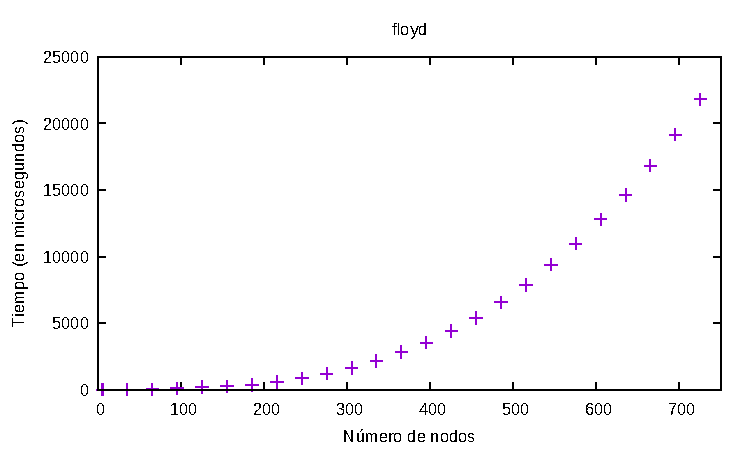
\includegraphics[width=0.3\textwidth]{../data/asus/floyd-points.pdf}}
         \subfloat[HP]{
          \label{hp:floyd-emp}
           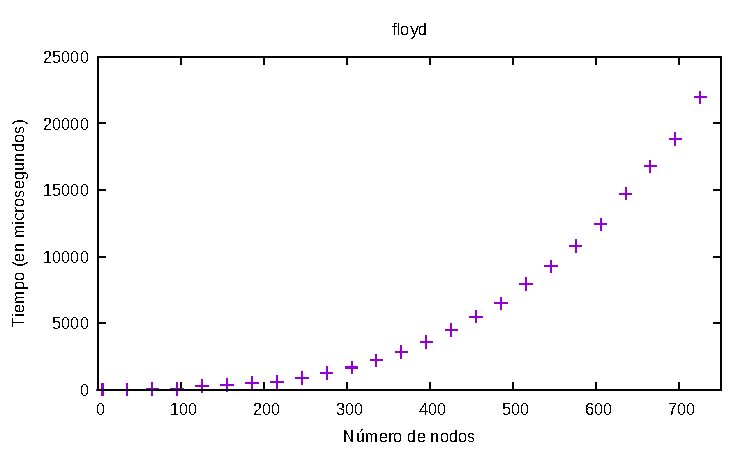
\includegraphics[width=0.3\textwidth]{../data/hp/floyd-points.pdf}}
         \subfloat[LENOVO]{
          \label{lenovo:floyd-emp}
           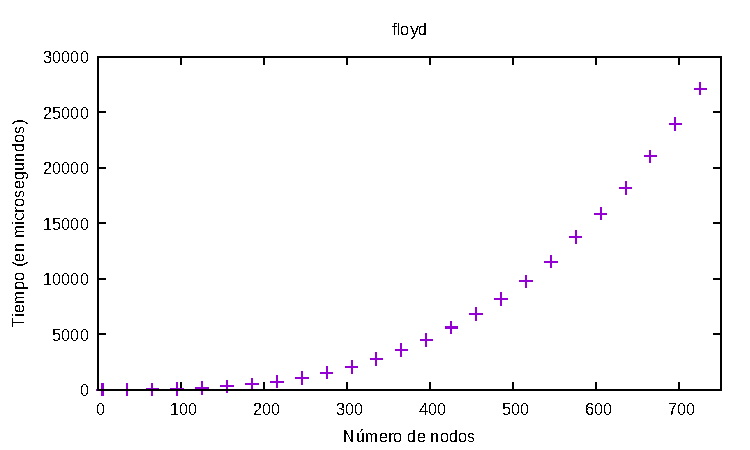
\includegraphics[width=0.3\textwidth]{../data/lenovo/floyd-points.pdf}}
        \caption{Representación gráfica de tiempos de ejecución del algoritmo Floyd.}
        \label{emp:floyd}
       \end{figure}

    \section{Eficiencia híbrida}
    
    En esta sección trataremos los datos obtenidos de la sección anterior mediante técnicas estadísticas para
    comprobar la consistencia de los datos experimentales con los calculados teóricamente. 

    \subsection{Algoritmo de inserción}
    \subsection{Algoritmo de selección}
    \subsection{Algoritmo HeapSort}
    \subsection{Algoritmo QuickSort}
    \subsection{Algoritmo de Floyd}

    
\end{document}